\documentclass[11pt]{article}
\usepackage[utf8]{inputenc}
\usepackage[T1]{fontenc}
\usepackage{fixltx2e}
\usepackage{graphicx}
\usepackage{longtable}
\usepackage{float}
\usepackage{wrapfig}
\usepackage{rotating}
\usepackage[normalem]{ulem}
\usepackage{amsmath}
\usepackage{textcomp}
\usepackage{marvosym}
\usepackage{wasysym}
\usepackage{amssymb}
\usepackage{hyperref}
\tolerance=1000
\usepackage{listings}
\usepackage{xcolor}
\usepackage[english, slovene]{babel}
\selectlanguage{slovene}
\author{Žiga Stopinšek}
\date{26. september 2014}
\title{Meshlab PHOV}
\hypersetup{
  pdfkeywords={},
  pdfsubject={},
  pdfcreator={Emacs 24.3.1 (Org mode 8.2.7c)}}
\begin{document}

\maketitle
\section{Opis orodja}
\label{sec-1}
Mehlab je programska oprema za ogledovanje, urejanje, manipuliranje in izvažanje 3D modelov. Sam po sebi
ne omogoča fotogrametrije, vendar pa že vsebuje orodje Arc3D, ki omogoča ogledovanje in urejanje
fotogrametričnih oblakov točk, pridobljenih s spletno storitvijo Arc3D. Problem, ki ga rešuje
orodje Meshlab PHOV je nalaganje in obdelava fotografij izključno v orodju Meshlab.

Arheologom po svetu je programska oprema Meshlab blizu, organiziranih pa je tudi vrsto delavnic za
spoznavanje s programom, tudi v Sloveniji. Zato bi integracija takšnega orodja v že nek poznan
program uporabniku olajšala proces spoznavanja in učenja novega orodja.

\section{Uporaba orodja}
\label{sec-2}
Uporabniški vmesnik za uporabo PHOV orodja v Meshlabu je izjemno preprost, zaradi česar pa je težje sistem
prilagajati. Vsa komunikacija s storitvijo poteka preko gumba za orodje, ki ima v različnih okoliščinah
različen pomen. 

\begin{figure}[!htbp]
\centering
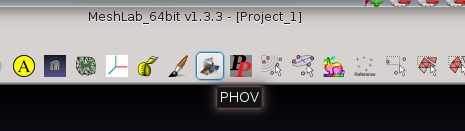
\includegraphics[width=5cm]{./icon.png}
\caption{\label{fig:icon}Gumb PHOV}
\end{figure}

\subsection{Nalaganje modela}
\label{sec-2-1}
Zaradi preprečevanja napadov je možno procesirati le en set fotografij na enkrat. To storimo s pritiskom
gumba PHOV. Vmesnik, če dobi od strežnika dovoljenje, omogoči nalaganje fotografij. Po vsakem nalaganju
nas vmesnik vpraša, če želimo končati. Če odgovorimo z NE, je mogoče ponovno nalagati sete fotografij, sicer
pa vmesnik sporoči strežniku ukaz za procesiranje.

\begin{figure}[!htbp]
\centering
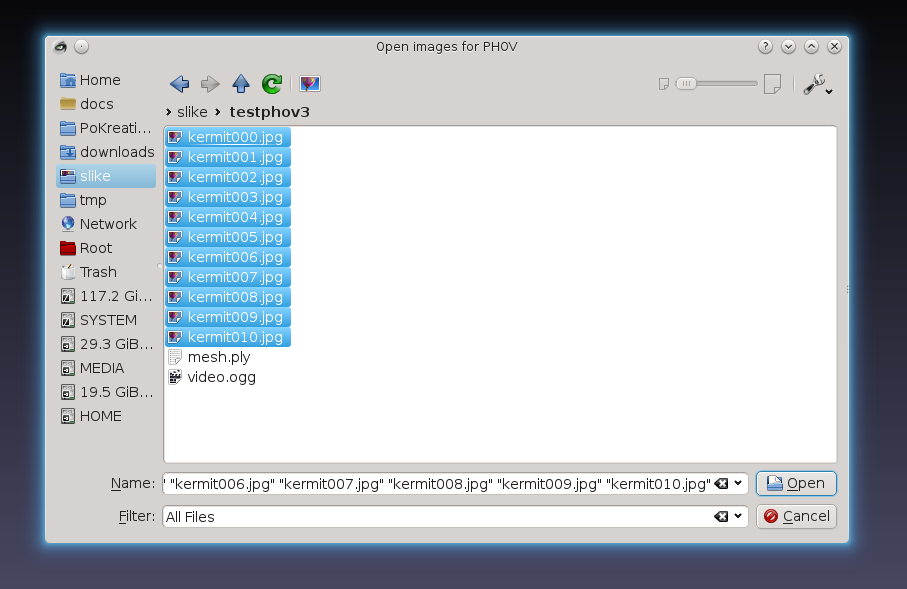
\includegraphics[width=8cm]{./images.png}
\caption{\label{fig:images}Nalaganje slik}
\end{figure}

\begin{figure}[!htbp]
\centering
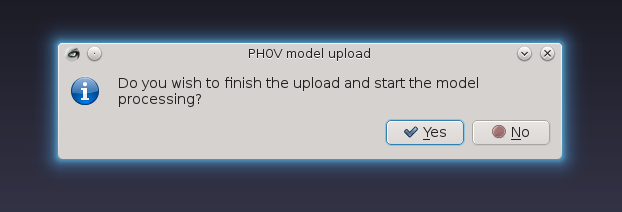
\includegraphics[width=5cm]{./uploadother.png}
\caption{\label{fig:uploadother}Dodatno nalaganje}
\end{figure}

\subsection{Čakanje na rezultat}
\label{sec-2-2}
Zaradi omejitev pri razvoju v okolju Meshlab mora uporabnik sam zahtevati pregled rezultata. S klikom na
tipko PHOV zahteva poizvedovanje na strežniku. Možne so tri različne posledice:
\begin{itemize}
\item sporočilo "model je še v obdelavi"
\item sporočilo "obdelava ni bila uspešna", vse operacije se prekličejo, uporabnik mora poskusiti znova
\item dialog za shranjevanje rezultata 3D modela
\end{itemize}

\begin{figure}[!htbp]
\centering
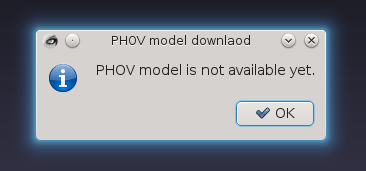
\includegraphics[width=5cm]{./waiting.png}
\caption{\label{fig:waiting}Čakanje na rezultat}
\end{figure}

\begin{figure}[!htbp]
\centering
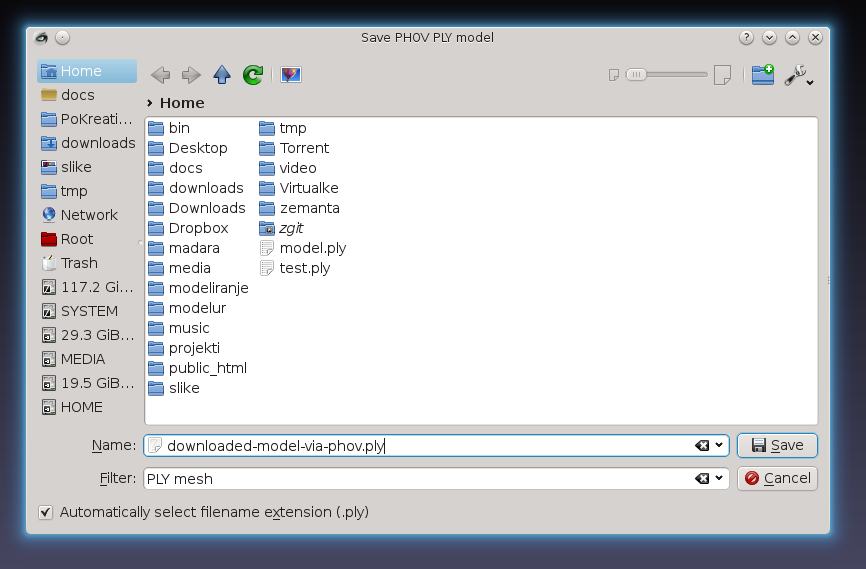
\includegraphics[width=8cm]{./download.png}
\caption{\label{fig:download}Prenos modela}
\end{figure}

\begin{figure}[!htbp]
\centering
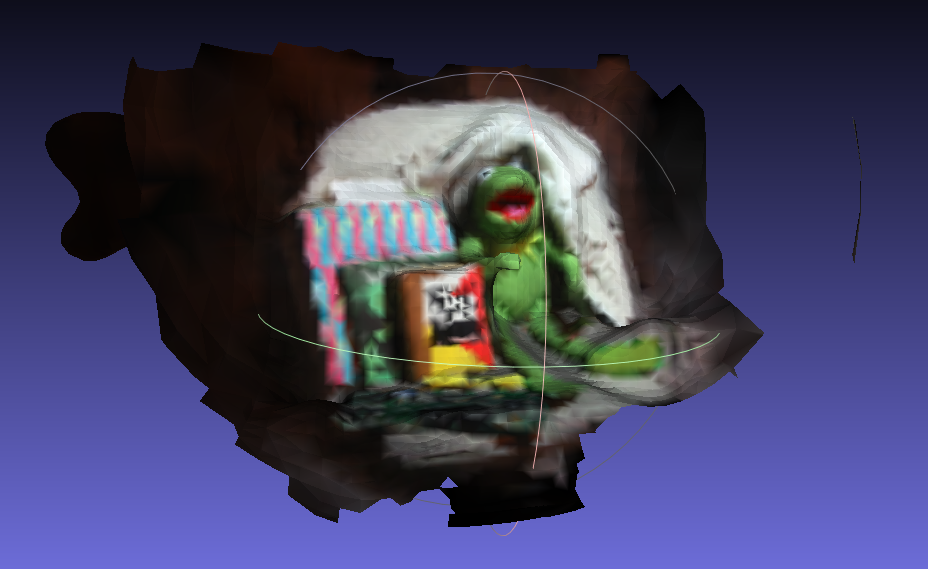
\includegraphics[width=8cm]{./model.png}
\caption{\label{fig:model}Pridobljeni 3D model}
\end{figure}

Ko prenesemo 3D model na računalnik, ga lahko po utečeni metodi
uvozimo v projekt.

\section{Namestitev}
\label{sec-3}
Ker orodje še ni na seznamu podprtih orodij, je potrebo za uporabo
orodja program prevesti ročno na računalniku. Za prevajanje kode na
računalniku so priložena navodila že znotraj izvorne kode programa
Meshlab. 

Za vključitev orodja je potrebno:
\begin{itemize}
\item v datoteko \emph{meshlab\_full.pro} dodati za vrstico, ki vsebuje \emph{edit\_arc3D}, dodati vrstico z vsebino:o \emph{meshlabplugins/edit\_phov $\backslash$}
\item v direktorij \emph{meshlabplugins} je potrebno skopirati izvorno kodo orodja
\end{itemize}

\section{Dokumentacija kode}
\label{sec-4}
Vsa logika programa se nahaja v datoteki \emph{edit\_phov.cpp}. Datoteka \emph{edit\_phov\_factory.cpp} je nujno potrebna le za inicializacijo orodja. 
Vsebina \emph{header} datotek:
\begin{itemize}
\item \emph{edit\_phov\_api.h.template} vsebuje iskalne nize (regex) in URL naslove do API-ja. Za delovanje jo je potrebno preimenovati in vnesti prave URL naslove.
\item \emph{edit\_phov\_factory.h} vsebuje meta podatke za nalaganje orodja.
\item \emph{edit\_phov.h} vsebuje meta podatke za izvajanje kode.
\end{itemize}

\subsection{Dokumentacija najpomembnejših funkcij}
\label{sec-4-1}
Najpomembnejše funkcije so naslednje:
\begin{itemize}
\item \emph{StartEdit} - potek orodja
\item \emph{loadSettings} - nalaganje nastavitev iz INI datoteke
\item \emph{saveSettings} - shranjevanje nastavitev v INI datoteko
\item \emph{getPhovId} - pridobitev ID 3D modela
\item \emph{checkDownloadAvailable} - preveri, ali je 3D model že na voljo oz. če je prišlo do napake
\item \emph{downloadModel} - iz spleta prenese 3D model
\item \emph{uploadImages} - nalaganje fotografij
\item \emph{finishUpload} - zaključi nalaganje fotografij
\item \emph{deleteModel} - brisanje modela, kar pa trenutno še ni podprto
\end{itemize}

Vsi zahtevki se delajo na roke. Primer zahtevka za pridobitev ID:
\begin{lstlisting}
void EditPhovPlugin::getPhovId() {
    QNetworkAccessManager nm(this); QEventLoop eventLoop;
    QUrl url(apiUrlGetId);
    QByteArray postData;
    postData.append("notify=mailto:example@email.com");
    QNetworkRequest request(url);    
    request.setHeader(QNetworkRequest::ContentTypeHeader, 
                      "application/x-www-form-urlencoded");
    QObject::connect(&nm, SIGNAL(finished(QNetworkReply*)),
                     &eventLoop, SLOT(quit()));
    QNetworkReply* reply = nm.post(request, postData);
    eventLoop.exec(); 
    if (reply->error() == QNetworkReply::NoError) {
        QRegExp rgx(rxId);
        int pos = rgx.indexIn(reply->readAll());
        if (pos > -1) {
            phovID = rgx.cap(1);
            saveSettings();
        } else {}
    } else {}
    delete reply;
}
\end{lstlisting}
% Emacs 24.3.1 (Org mode 8.2.7c)
\end{document}